\chapter{绪论}\label{chap:introduction}

\section{概述}
\subsection{稀疏建模:时代的需要}
获取信息,从而认识大千世界,是人类文明发展的主旋律。在目前智能时代,信息时代的发展过程中,各种传感器技术快速发展,数量不断增长,硬件成本减低,数据量呈现爆炸式增长。数据洪流给传统的数据存储,传输处理方法带来了巨大的压力。海量数据促使新的方法:从数据中学习,形成信号表达,信号获取与复原的新概念和新方法。

自然界的大多数信号具有一定的结构性,结构性信号的自由度要远低于信号本身的维度。海量数据的典型特征就是信息冗余,其携带的信息量非常有限。可以用稀疏性来描述这个特性。

信息表达的研究表明,几乎在所有的情况下,数据中携带的信息量是稀疏的。
可以说稀疏性是海量数据的本质特性之一,正是这个特性,为海量数据的的表达和处理提供了便利,为更有效的数据解译提供了可能。

信号表达的基本任务是描述信号组成的基本要素,揭示信号组织和生成的方式。离散余弦变换和小波变换等经典信号仅描述了信号的基本要素和简单线性组织方法,不能揭示信号深层次的组织和生成方式。

在统计分析和机器学习的驱动下,从数据中学习信号特征的表达方法开始出现,信号表达进入基于学习的表达方法中。

\subsection{稀疏建模的哲学基础:剃刀原则}
稀疏建模,是节省性原则在现代统计学,机器学习和信号处理领域的特殊体现。在这些领域,一个基础性的问题就是,由于观测成本或其他限制,需要从数量相对较少的观测中对未观测高维信号进行精确复原。

一般的,高维小样本推断问题是欠定的,且在计算上是难以处理的,除非该问题具有某一特定的结构,例如稀疏性。

事实上,当仅有少量变量为真正重要的变量时,真实解可以很好的由稀疏向量来近似,将剩余变量设置为0或者接近0。换言之,少量最相关的变量(起因,预测因子等),通常对于解释感兴趣的现象来说是充分的。

更一般的,即使原始问题没有产生稀疏解,我们可以找到一个映射(或字典),将其映射到新的坐标系统,从而实现稀疏表示。因此稀疏机构看上去是很多自然信号固有的性质,没有该结构,认知并适应这个世界是相当具有挑战性的问题。

\section{问题的提出}
如何从有限的观测中推断出未被观测到的高维“世界状态”,这个问题常常出现在广泛的实际应用中。



\begin{enumerate}
	\item 寻找基因中引发某种疾病的子集;
	\item 定位与某一心理状态存在关联的大脑区域	
	\item 诊断大规模分布式计算机系统中的性能瓶颈
	\item 使用压缩观测值重构高质量的图像
\end{enumerate}

更一般的例子是,从任意一类信号的含噪编码中对信号解码,以及在高维但小样本的统计情况下估计模型参数。

图xx描述的就是这种基本推断难问题,其中$x=(x_1,x_2,\cdots,x_n)$代表一个未被观测的n维的世界状态,$y=(y_1,y_2,\cdots,y_m)$代表它的m个观测结果。观测结果的输出向量y可以看成是输入向量x的一个含噪函数(编码)。
\begin{figure}[th]
	\centering
	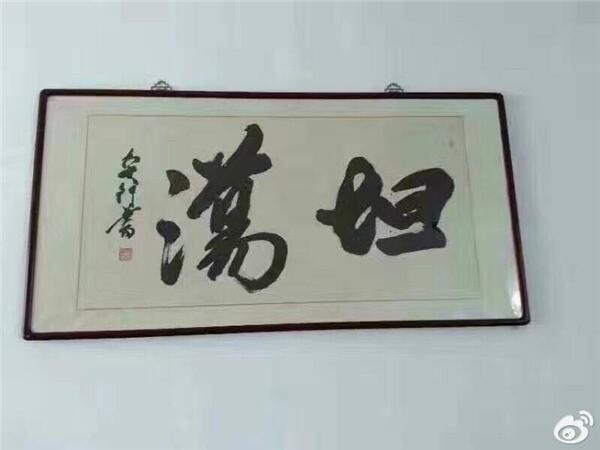
\includegraphics[width=0.5\linewidth]{Img/Chap_Intro/fig1_1}
	\caption[hello]{hellohello}
	\label{fig:test}
\end{figure}
一种常用的推断(解码)方法是,给定观测结果y,找到某种损失函数$L(x;y)$,使之最小化得到x。例如常见的极大似然法,就是旨在找到一个使得观测结果的似然$P(y|x)$最大化的参数向量x。

然而在许多实际问题中,未被观测到的变量在数量上远远多于观测值,因为对真实世界的观测成本很高,且受到具体问题的限制。通常未知变量的总数可能达到数千个或上百万个,而观测结果或者样本数量总数通常只有几百个。因此上述似然表达式将变为欠定情况。

同时,为了限定可能的解空间,必须引入额外的,反映了特定领域性质或假设的正则化约束。从贝叶斯概率的假设来说,正则化可以看做是对未知参数四家了先验$P(x)$,然后最大化后验概率$P(x|y)=P(y|x)P(x)/P(y)$。

或许,关于问题结构做的最简单、最常见的假设之一是解为稀疏的。换言之,通常假定在特定情况下,只有一个相对较小的变量子集是真正重要的。例如:
\begin{itemize}
	\item 一个系统只出现少量的并发故障;
	\item 只需要少数非零傅里叶系数就能满足对不同信号类型的准确表示;
	\item 只有一小部分预测变量(如基因)与响应变量(疾病或特征)最相关;
	\item 学习某一精确预测模型也只需要一小部分预测变量。
\end{itemize}
在这些例子中,我们寻求的解可以看成是一个仅有少量非零坐标的稀疏高维向量。这一假设与哲学中的节省性原则一致,而这一原则通常被称为奥卡姆剃刀原则,由中世纪著名哲学家奥卡姆威廉提出。之前可追溯到亚里士多德和托勒密,之后也出现了许多关于节省性原则的阐述,其中包括牛顿的著名表述:“寻求自然事物的本因,只需找到真实而又足以解释其现象即可,无需更多。”


\subsection{欠定线性系统}

线性代数的可用于对对线性方程组求,对该问题进行彻底考查。而线性方程组求解是很多工程应用和解决方案的核心问题。令人惊讶的是,在这个问题中,却有一个不得不用线性系统的稀疏解来解决的初级问题,该问题最近才被深入的探索和研究。

{\heiti 
我们会发现这个解有很令人惊讶的答案,它促进了很多的实际发展。在这一章中我们应该集中精力认真的定义这个问题,为在以后的章节中的问题答案做好准备。}


设有一个矩阵$A\in R^{n\times m}(n<m)$,定义一个由线性方程组$Ax=b$描述的\emph{欠定系统}。该欠定系统中,未知数多于方程式数目。如果向量b不在矩阵A列向量张成的空间中,则这个系统无解。否则,方程有无穷多个解。为避免这种异常情况发生,本书中假设A为一个满秩矩阵,既其列向量张成整个$R^n$空间。

这种欠定线性系统求解的问题,我们在工程中常常碰到。例如:
{\heiti
图像处理中的上采样问题,一副未知图像x经过模糊和下采样,将得到一副低质量小图像b。矩阵A代表了这种退化操作。我们的目标就是从观测b中重构出原始图像x。
}
显然,有无数中图像x能用来解读降质图像b,但其中总有一些看起来更好一些,问题是我们怎么去寻找最好,最合适和最准确的x呢?


\subsection{正则化解}
在上面的例子中,我们总希望得到唯一解,但我们面临的最大障碍是,其可能存在无穷解。为了将选择范围缩小为一个满意解,显然需要增加条件。

一个常用的增加条件的方法,就是正则化(regularization),即引入一个对x的候选解进行合理性评价的函数$J(x)$,并期望其值越小越好,对常规的优化问题$(P_J)$可做如下定义:
\begin{equation}
	(P_J):\quad  \min_{x}J(x)\quad s.t.\quad b=Ax
\end{equation}
\par 现在可用$J(x)$来约束可能解的类型。如在图像上采样用,一般用$J(x)$表征$x$的光滑度,或分段光滑度。

但最常见的J(x)函数是欧式范数的平方$\Vert{x}\Vert^2_2$。事实上这种选择带来的$(P_2)$问题存在唯一解$\hat{x}$。可利用拉格朗日法对其求解。

定义拉格朗日公式:
\begin{equation}%\label{key}
L(x)= \Vert x \Vert_2^2 + \lambda^{T}(Ax-b)
\end{equation}

这里$\lambda$为约束集合所对应的拉格朗日乘子。将上式两边对$ \lambda $求导可得:
\begin{equation}\label{key}
\frac{\partial L(x)}{\partial\lambda}= 2 x  +A^{T}\lambda 
\end{equation}

令其等于0,由此得到解如下:
\begin{equation}\label{key}
\hat{x}_{opt} = -\frac{1}{2} A^T \lambda
\end{equation}

将这个 解带入约束条件$ Ax=b $,可得:
\begin{equation}\label{key}
A\hat{x}_{opt} = -\frac{1}{2} A A^T \lambda = b  \Longrightarrow
 \lambda = -2(AA^T)^{-1}b 
\end{equation}

再将该结果带入式1-4,就可以得到常见的闭合形式的伪逆解:
\begin{equation}\label{key}
\hat{x}_{opt} = -\frac{1}{2} A^T \lambda = A^{T}(AA^T)^{-1}b  = A^{+}b
\end{equation}


欧式范数被广泛的应用于各个工程的领域,主要在于其比较简单,可以给出上述闭合形式的唯一解。在信号和图像处理中,这种正则化处理被广泛应用于各种逆问题求解,信号表示等领域。但其并不是真正的最佳选择。





































\section{稀疏表示的研究概况}

过去几年,稀疏性相关研究已经远远超出了原来信号复原理论描述的范畴,涵盖了:
\begin{enumerate}
	\item 稀疏非线性回归,如广义线性模型
	\item 稀疏概率网络,如马尔科夫网络和贝叶斯网络
	\item 稀疏矩阵分解,如字典学习
	\item 稀疏主成分分析,
	\item 稀疏非负矩阵分解
	\item 稀疏贝叶斯学习
\end{enumerate}


此外,由于稀疏建模领域存在大量的新进展,一些重要的问题例如低秩矩阵完备,在很多应用中出现,包括协同过滤、度量学习、多任务学习等,由于秩最小化问题类似于$ \ell_0 $范数最小化,非常难以处理,通常可以通过迹范数(或称为核范数)来利用凸松弛,其中迹范数即为奇异值向量的$ \ell_1 $范数。


